\section{Makroskopowy opis własności elektronowych ośrodków materialnych}
\subsection{Makroskopowa elektrodynamika ośrodków materialnych}
\subsubsection{Podsumowanie}
Równania Maxwella w postaci makroskopowej (w ośrodkach materialnych) mają postać:
\begin{equation} \nabla \cdot \vec{D}\arg=\wp\arg \label{r1}
 \end{equation}
 
\begin{equation} \nabla \times \vec{H}\arg-\partial_t\vec{D}\arg=\vec{J}\arg \label{r2}
\end{equation}

\begin{equation} \nabla \times \E+\partial_t \B=\vec{0} \label{r3}\end{equation} 

\begin{equation} \nabla \cdot \B=0 \end{equation}
gdzie $\wp$ oznacza makroskopową gęstość ładunku, zdefiniowaną poprzednio jako: $\wp=<q_e\sum_i\delta(\r-\r_i(t))>+<\sum_nq_n\delta(\r-\r_n(t))$

wn.1. Makroskopowe pola $\E,\B$ są wartościami średnimi pól mikroskopowych $\vec{e},\vec{b}$. Są to pola pierwotne, natomiast pola $\vec{D},\vec{H}$ są polami wtórnymi wynikającymi z ustalonej procedury średniowania.

\subsubsection{Zasada zachowania ładunku}
\begin{enumerate}
\item{Ogólne wyprowadzenie}\\
Lokalnie (czyli w ośrodku) jest spełniona zasada zachowania ładunku, tzn. zmiana gęstości ładunku w ograniczonym obszarze $\Omega$ jest spowodowana przepływem prądu przez powierzchnię zamkniętą $\partial\Omega$ otaczającą ten obszar.
\begin{center}
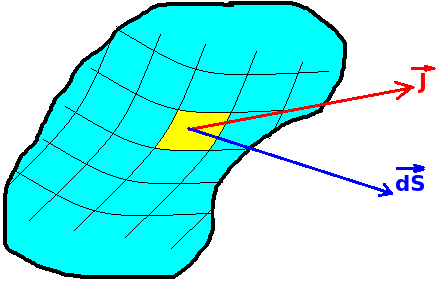
\includegraphics[width=6cm] {obrazek1}
\end{center}
\textit{Rys. 1. Rysunek pomocniczy.}
Spełnione jest:
\begin{equation}
\frac{dQ}{dt}=-\int \vec{dS}\cdot\vec{J}\arg \label{zl}
\end{equation}
gdzie: 
\begin{itemize}
\item $\vec{dS}$ - element powierzchni; $|\vec{dS}|$ - pole powierzchni
\item Q- całkowity ładunek, wyrażający się wzorem:
\begin{equation}Q(t)=\int d^3r \rho\arg \label{Q} \end{equation}
\item $\vec{dS}$  - wektor powierzchni, którego długość jest równa polu powierzchni, 
\item natomiast wyrażenie po prawej stronie to natężenie prądu będące równe strumieniowi przepływającemu przez daną powierzchnię:
\begin{equation}
I(t)=\int \vec{dS}\cdot\vec{J}\arg 
\end{equation}
\end{itemize}
uw. Minus w równaniu (\ref{zl}) oznacza, że ładunek może tylko wypływać spod powierzchni.\\
uw2. Wyrażenie pod całką to strumień prądu płynący przez rozważany obszar.

Wstawmy równanie (\ref{Q}) do równania (\ref{zl}):
\begin{equation}
\partial_t \int_{\partial\Omega} d^3r\rho\arg= -\int_{\partial\Omega}\vec{dS}\cdot\vec{J}\arg 
\stackrel{\text{tw.Gaussa}}{=} -\int_\Omega d^3r\nabla\cdot\vec{J}\arg
\end{equation}
\begin{equation}
\int d^3r\{\partial_t \rho\arg+\nabla \cdot\vec{J}\arg\}=0
\end{equation}
Stąd:
\begin{equation}
\partial_t \rho\arg+\nabla \cdot\vec{J}\arg=0 \label{zl2} \end{equation}
Wzór (\ref{zl2}) to prawo zachowania ładunku - ładunek nie może zniknąć, może tylko przepłynąć przez powierzchnię.

\item{Wyprowadzenie praw zachowania ładunku z praw Maxwella}\\
Zadziałajmy obustronnie $\partial_t$ na 1. równanie Maxwella (\ref{r1}) oraz $\nabla\cdot$ na 2. równanie Maxwella (\ref{r2}):
\begin{equation}
(1)~~\Rightarrow ~~\partial_t \nabla\cdot \vec{D}\arg=\delta_t \rho(\r,t) ~~\Rightarrow~~ \nabla\cdot[\partial_t\vec{D}\arg=\partial_t\rho\arg \end{equation}
 \begin{equation}
 (2)~~\Rightarrow~~ \underbrace{\nabla\cdot[\nabla\times\vec{H}\arg]}_{=0 \text{ (bo jest to div z rot)}}-\nabla\cdot\partial_t\vec{D}\arg=\nabla\cdot\vec{J}\arg
\end{equation}
Łącząc oba te równania dostajemy:
\begin{equation}
-\partial_t\rho\arg=\nabla\cdot\vec{J}\arg \label{zz}
\end{equation}
Równanie (\ref{zz}) to zasada zachowania ładunku.

\item{Równania materiałowe} \\
Z jednej strony równania Maxwella są niezmiennicze względem zmiany ośrodka, z drugiej strony ich rozwiązania- pola $\E,\B$- są różne w różnych ośrodkach. Dlatego potrzebujemy dodatkowych równań, które będą określać ośrodek- dlatego postulujemy równania materiałowe:
\begin{equation} {D}_i\arg=\sum_{j/1}^3\int d^3r'\int_{-\infty}^t dt' \epsilon_{ij}\argg E_j \label{rm1}\end{equation}
\begin{equation} H_i \arg =\sum_{j/1}^3\int d^3r'\int_{-\infty}^t dt' \mu^{-1}_{ij}\argg B_j \label{rm2}\end{equation}
\begin{equation} J_i \arg =\sum_{j/1}^3\int d^3r'\int_{-\infty}^t dt' \sigma_{ij}\argg E_j \label{rm3}  \text{ - mikroskopowe prawo Ohma}\end{equation}
\begin{verse}\textbf{wn.1.} Mamy zatem zestaw równań: Równania Maxwella+równania materiałowe \end{verse}
\begin{verse}\textbf{wn.2.} W równaniach materiałowych jądrem całkowym są:\\
(\ref{rm1}): ~ $\epsilon_{ij}\argg$ - to element tensora przenikalności elektrycznej ośrodka\\
(\ref{rm2}):  ~$\mu^{-1}_{ij}\argg$ - to element tensora odwrotności przenikalności magnetycznej\\
(\ref{rm3}):  ~$\sigma_{ij}\argg$  - to element tensora przewodnictwa elektrycznego. \end{verse}
\begin{verse} \textbf{uw.1.} Równania materiałowe mają swoje uzasadnienie w termodynamice stanów nierównowagowych, natomiast do elektrodynamiki zostały dodane \textsl{ad hoc}.
uw.2. \end{verse}
\begin{verse} \textbf{uw.2.} Ostatnie (\ref{rm3}) równanie to mikroskopowe (lokalne) prawo Ohma, które można również zapisać w popularniejszej wersji:
\begin{equation} \vec{J} \arg =\sigma\arg E\arg \end{equation} \end{verse}

\item{Równania Maxwella a prąd stały}\\
\begin{verse} \textbf{Zał.} Załóżmy, że \textbf{prąd jest stały}, tzn. płynie w sposób ciągły i nie gromadzi się (jest stały w czasie). \end{verse}

Wówczas:\begin{itemize}
\item Równanie Maxwella (\ref{r2}) $\Rightarrow$ powstaje stałe pole $\vec{H}$
\item Równanie Maxwella (\ref{r3}) $\Rightarrow ~~ \nabla\times\vec{E}(\r)+\underbrace{\partial_t\vec{B}(\r)}_{=0}=0$ \\
Stąd:
\begin{equation} \nabla\times\vec{E}(\r)=0 \end{equation}
Ponieważ wiemy, że dywergencja z rotacji daje 0, to $\vec{E}$ musi dać się przedstawić jako:
\begin{equation} \vec{E}=-\nabla V(\r) \label{Epot}\end{equation}
gdzie $V(\r)$ to potencjał.
\begin{verse} \textbf{wn.} Jeśli prąd jest stały, to pole elektryczne ma potencjał. \end{verse} 
\item Prawo zachowania ładunku (\ref{zl2}) $\Rightarrow ~~ \underbrace{\partial_t\rho\arg}_{=0}+\nabla\cdot\vec{J}\arg=0 $
\begin{equation} \nabla\cdot\vec{J}({\r})=0 \end{equation}
\item Mikroskopowe prawo Ohma $\Rightarrow ~~ \nabla[\sigma(\r)\vec{E}(\r)]=0$ \\
Łącząc to równanie z równaniem (\ref{Epot}), dostajemy: \\ 
\begin{equation} -\nabla \cdot[\sigma(\r) \nabla V(\r)] =0  \nonumber \end{equation}
\begin{equation} \nabla \cdot[\sigma(\r) \nabla V(\r)] =0 \label{doLaplace} \end{equation}
\item Załóżmy teraz, że przewodnictwo jest wszędzie takie samo: $\sigma(\r)=const=\sigma $.\\
Wówczas z równania (\\ref{doLaplace}) wynika:
\begin{equation} \sigma \nabla ^2 V(\r) =0 \end{equation}
O ile $\sigma \neq 0 $ (czyli nie jest to izolator):
\begin{equation} \nabla^2 V(\r)=0\end{equation}
Jest to równania Laplace'a.
\begin{verse} \textbf{wn.} Jeśli prąd jest stały, to potencjał układu spełnia równanie Laplace'a. \end{verse}
\begin{verse} \textbf{uw.} Bez założenia o prądzie stałym dostalibyśmy równanie Poissona \end{verse}
\end{itemize}

\begin{verse}{\textbf{Dygresja} - potencjał a energia potencjalna}
Energia potencjalna wyraża się wzorem:
\begin{equation} U(\r) \equiv \int d^3r'\rho(\r')V(\r) \end{equation}
Łącząc powyższe równanie z definicją gęstości ładunkowej:
\begin{equation} U(\r) = \int d^3r'q\delta(\r-\r')V(\r)\end{equation}
Stąd:
\begin{equation} U(\r) = qV(\r) \label{Pot}\end{equation}
Równanie (\ref{Pot}) to związek pomiędzy energią potencjalną a potencjałem.
\end{verse}
\end{enumerate}
\subsection{Zlinearyzowane relacje konstytutywne ośrodków materialnych}
\subsubsection{Ogólna postać równań materiałowych}
Można zauważyć, że wszystkie równania materiałowe (\ref{rm1}),(\ref{rm2}),(\ref{rm3}) mają postać:
\begin{equation} \vec{Y}(\r,t)=\int d^3r \int_{-\infty}^t dt' \hat{\chi}(\r,\r',t,t') \vec{X}(\r',t') \end{equation}
lub równoważnie:
\begin{equation} {Y}_i(\r,t)=\sum_{j/1}^3 \int d^3r \int_{-\infty}^t dt' {\chi}_{ij}(\r,\r',t,t') X_j(\r',t') \end{equation}
gdzie:\\
\begin{itemize} \item $\vec{Y}$ - wektor reprezentujący pole wtórne
\item $\vec{X}$ - wektor reprezentujący pole pierwotne
\item $\hat{\chi} $ - to tzw. uogólniona podatność (inaczej: funkcja odpowiedzi układu). Jest to tensorowe jądro całkowe, służące do przekształcenia pola pierwotnego we wtórne - zatem wnosi ona informację o ośrodku.
\end{itemize}
\begin{verse}\textbf{uw.}
Dlaczego całka po czasie biegnie do $t$ a nie do $\infty$? \\
Ponieważ wówczas $\chi$ zbiera informacje do chwili obecnej. Gdyby całka była do $\infty$, to złamalibyśmy \textbf{zasadę przyczynowości} (wyraża ona, że skutek obserwowany w chwili obecnej zależy tylko do przyczyn z przeszłości). \\
Można zatem postawić:
\begin{equation}\chi_{ij}(\r,\r',t,t')=0 \text{ ~~~~dla~ } t'>t\end{equation}
\end{verse}

\subsubsection{Równania materiałowe a teoria liniowej odpowiedzi}
\textbf{Fakty:}
\begin{enumerate}
\item Pola wtórne są liniowymi funkcjonałami pól pierwotnych:
\begin{equation} \vec{Y}[\alpha_1\vec{X}_1 + \alpha_2\vec{X}_2]=\alpha_1 \vec{Y}[\vec{X}_1] + \alpha_2 \vec{Y}[\vec{X}_2] \end{equation}
\textbf{uw.} Jeśli uciąglimy tę sumę, dostaniemy całkę.
\item Równania materiałowe pozostają słuszne, jeśli pola pierwotne można traktować jako słabe zaburzenia. Wówczas można rozwinąć w szereg McLaurina:
\begin{equation}\vec{Y}[\vec{X}]=\vec{Y}[\vec{0}]+ \frac{\delta\vec{Y}}{\delta\vec{X}}|_{\vec{0}}\vec{X} + \frac{1}{2}\frac{\delta^2 \vec{Y}}{\delta\vec{X}^2}|_{\vec{0}}\vec{X}^2 + ...\end{equation}
gdzie: $\vec{Y}[\vec{0}]=0$ (bo nie może istnieć pole wtórne bez pierwotnego), zatem:
\begin{equation}[\vec{X}]=\vec{Y}[\vec{0}]+ \frac{\delta\vec{Y}}{\delta\vec{X}}|_{\vec{0}}\vec{X} + \mathcal{O}(\vec{X}^2)\end{equation}
\end{enumerate}
\textbf{Założenie:}\begin{verse} 
Załóżmy, że pola wtórne są proporcjonalne do pól pierwotnych (tzw. linearyzacja równania). Wówczas:
\begin{equation}\vec{Y}[{\vec{X}}] \simeq \frac{\delta\vec{Y}}{\delta\vec{X}}|_{\vec{0}} \vec{X} = \hat{\mathcal{L}}\vec{X}\end{equation} \end{verse}
Ostatecznie więc:
\begin{equation}\vec{Y}[{\vec{X}}] = \hat{\mathcal{L}}\vec{X} \label{RFen} \end{equation}
To przybliżenie nazywamy \textbf{teorią liniowej odpowiedzi}, zaś samo równanie (\ref{RFen}) - równaniem fenomenologicznym, a współczynniki $\hat{\mathcal{L}}$ - współczynnikami fenomenologicznymi. Współczynniki te dostajemy z doświadczeń i następnie staramy się je wyjaśnić za pomocą teorii.

\subsubsection{Uogólnienie na wiele pól zaburzających - zjawiska krzyżowe}
Z racji liniowości wektora $\vec{Y}$, równanie (\ref{RFen}) można uogólnić na wiele pól zaburzających (np. możemy jednocześnie rozważać pola $\B$ i $\E$) :
\begin{equation} \vec{Y}=\hat{\mathcal{L}}\vec{X} \arg 
\stackrel{\text{uogólnienie}}{\longrightarrow}  {Y}_i=\sum_{j/1}^n \mathcal{L}_{ij} X_j \end{equation}
\begin{verse} \textbf{Np.} Niech n=2. Wówczas:
\begin{center} 
$\begin{cases} \vec{Y}_1=\mathcal{L}_{11}\vec{X}_1+\mathcal{L}_{12}\vec{X}_2 ~~~~~~~~~~/\mathcal{L}_{12}^{-1}\\ \vec{Y}_2=\mathcal{L}_{21}\vec{X}_1+\mathcal{L}_{22}\vec{X}_2 ~~~~~~~~~~/\mathcal{L}_{22}^{-1}
\end{cases}$
\end{center}

\textbf{wn.} Pole wtórne wynika z obu pól pierwotnych.\\
Wyznaczamy $\vec{X}_1$:
\begin{center}
$\begin{cases} \mathcal{L}_{12}^{-1}\vec{Y}_1=\mathcal{L}_{12}^{-1}\mathcal{L}_{11}\vec{X}_1+\vec{X}_2 \\ \mathcal{L}_{22}^{-1}\vec{Y}_2=\mathcal{L}_{22}^{-1}\mathcal{L}_{21}\vec{X}_1+\vec{X}_2 
\end{cases}$
\end{center}
Odejmując stronami, dostajemy:
\begin{equation} \mathcal{L}_{12}^{-1}\vec{Y}_1 - {L}_{22}^{-1}\vec{Y}_2 = [\mathcal{L}_{12}^{-1}\mathcal{L}_{11} - \mathcal{L}_{22}^{-1}\mathcal{L}_{21}]\vec{X}_1 \nonumber \end{equation}
\begin{equation} 
 [\mathcal{L}_{12}^{-1}\mathcal{L}_{11}-\mathcal{L}_{22}^{-1}\mathcal{L}_{21}]^{-1} \mathcal{L}_{12}^{-1}\vec{Y}_1 -   
 [\mathcal{L}_{12}^{-1}\mathcal{L}_{11} - \mathcal{L}_{22}^{-1}\mathcal{L}_{21}]^{-1} \mathcal{L}_{22}^{-1}\vec{Y}_2 =\vec{X}_1  \nonumber \end{equation}
 
\textbf{wn.} Pole pierwotne $\vec{X}_1$ można przedstawić w postaci kombinacji liniowej pól wtórnych, przy czym $\vec{X}_1$ produkuje $\vec{Y}_1$ oraz $-\vec{Y}_2$. Zauważmy, że $\vec{Y}_2$ jest z minusem, bo przeciwdziała ono polu $\vec{Y}_1$.\\ ~~~~Takie procesy z polami $\vec{Y}_1$ i $\vec{Y}_2$ naz. zjawiskami krzyżowymi.\\
\textbf{np.} W zjawiskach termoelektrycznych polami tymi są $\vec{E}$ i gradient temperatury $\nabla T$: Pole elektryczne przemieszcza elektrony, ale przez opór materiał się grzeje, więc powstaje gradient temperatury.
\end{verse}
\subsubsection{Klasyfikacja materiałów ze względu na jądro całkowe równania materiałowego}
\begin{enumerate}
\item Ośrodek materialny jest \textbf{lokalnie liniowy} wtedy i tylko wtedy, gdy $\hat{\chi}$ ma postać:
\begin{equation}\hat{\chi}(\r,\r',t,t')=\hat{\chi}(\r',t,t')\delta(\r-\r')\end{equation}
\item Ośrodek materialny jest \textbf{przestrzennie jednorodny} wtedy i tylko wtedy, gdy $\hat{\chi}$ ma postać:
\begin{equation}\hat{X}(\r,\r',t,t')=\hat{\chi}(\r-\r',t,t')\end{equation}
Jeśli równość ta nie zachodzi, to ośrodek jest \textbf{niejednorodny przestrzennie}.
\item Ośrodek materialny jest \textbf{czasowo jednorodny} wtedy i tylko wtedy, gdy $\hat{\chi}$ ma postać:
\begin{equation}\hat{\chi}(\r,\r',t,t')=\hat{\chi}(\r,\r',t-t')\end{equation}
 Np. gdy materiał się grzeje, to w różnych chwilach różne jest pole $\nabla T$
 Jeśli równość ta nie zachodzi, to ośrodek jest \textbf{niejednorodny czasowo}.
 \item Ośrodek materialny jest \textbf{czasowo i przestrzennie jednorodny} wtedy i tylko wtedy, gdy $\hat{\chi}$ ma postać:
\begin{equation}\hat{\chi}(\r,\r',t,t')=\hat{\chi}(\r-\r',t-t')\end{equation}
 Tę własność spełnia gaz elektronowy oraz nukleony w jądrze.
  \item Ośrodek materialny jest \textbf{izotropowy} wtedy i tylko wtedy, gdy elementy macierzowe $\hat{\chi}$ mają postać:
\begin{equation}{\chi}_{ij}(\r,\r',t,t')=\hat{\chi}(\r-\r',t-t')\delta_{ij}\end{equation}
 Jeśli równość ta nie zachodzi, to ośrodek jest \textbf{anizotropowy}.
 \item Ośrodek materialny jest \textbf{homogeniczny} wtedy i tylko wtedy, gdy elementy macierzowe $\hat{\chi}$ mają postać:
\begin{equation}{\chi}_{ij}(\r,\r',t,t')={\chi}\delta(\r-\r')\delta(t-t')\delta_{ij}\end{equation}
\end{enumerate}
\subsubsection{Równanie materiałowe dla ośrodka homogenicznego- konsekwencje}
Wróćmy do równania materiałowego:
\begin{equation} {Y}_i(\r,t)=\sum_{j/1}^3 \int d^3r \int_{-\infty}^t dt' {\chi}_{ij}(\r,\r',t,t') X_j(\r',t') \end{equation}
W ośrodku homogenicznym:
\begin{equation} {Y}_i(\r,t)=\sum_{j/1}^3 \int d^3r \int_{-\infty}^0 dt' {\chi}\delta(\r-\r')\delta(t-t')\delta_{ij} X_j(\r',t')\arg 
\stackrel{\text{tw.filtracyjne}}{=}\chi X_i(\r,t) \end{equation}
Zatem:\\
\begin{center}
%\caption{fsdF}
\begin{tabular}{|c||c|c|}
  \hline
 ${_Y^{~~X}}$ & $\vec{E}$ & $\vec{B}$\\
  \hline\hline
  $\vec{D}$ &  $\hat{\epsilon}$ & brak \\
\hline
  $\vec{H}$ &  brak & $\hat{\mu}^{-1}$ \\
  \hline
  $\vec{J}$ &  $\hat{\sigma}$ &  brak\\
    \hline
\end{tabular} 
\end{center}
\textbf{wn. 1.} Z powyższego wynika mikroskopowe prawo Ohma dla ośrodków homogenicznych: \begin{equation} \vec{J}(\r,t)=\sigma\E \end{equation}
Zatem Ohm miał szczęście, że przykładał małe pola (bo w powyższych rachunkach zastosowaliśmy rachunek zaburzeń prawdziwy dla małych pól).\\
\textbf{wn. 2.} Dla układów homogenicznych skalarna stała $\chi$ reprezentuje stałą materiałową, która opisuje w sposób ilościowy rozpatrywaną własność ośrodka.
\subsubsection{Punkt widzenia}
Ustalmy jeden z dwóch możliwych punktów widzenia:
prąd elektryczny jest konsekwencją przyłożonego pola elektrycznego $\E$. Pole elektryczne to przyczyna, a prąd to skutek.
